% Based on:
% Introduction and Overview of the Multics System
% F.J. Corbato (MIT)
% and 
% V.A. Vyssotsky (Bell Labs)

% multicians.org


% # --------------------------------------------------------------------------------- #
\section{History of Multics}

In the early 1960s, large scale-computing was dominated by \textit{mainframes}. Controlled by \textit{batch processing} 
supervisor program. Users submitted jobs on \textit{5 hole paper tape}, and received printed output.
Timesharing, in which a large machine switched between multiple users, giving each the impression of virtual computer, 
had been proposed by MIT Professor \textit{John McCarthy} in 1959.

\textbf{Multics} (Multiplexed Information and Computing Service) is a timesharing operating system which begun in 1965 and been 
used until 2000. The system was started as a co-project of MIT's \textit{Project MAC}, \textit{Bell Labs} (withdrew from development 
 in 1969) and \textit{General Electric Company}.

Chief of project was \textbf{Professor Fernando J.Corbató} (MIT). MIT operated a Multics timesharing service with over a thousand users 
through the 1970s. Major customer of this service was Honeywell, which also helped a lot during the \textit{security enhancement era} 
of Multics operating system.

Multics was invented to provide access to many remote terminal users simultaneously, in a manner similar to MIT's \textbf{CTSS} 
system. Multics combined ideas from other operating systems with new innovations. Security was a fundamental design requirement.
Multics ran on specialized expensive CPU hardware that provided a segmented, paged, ring-structured virtual memory. 

Multics was introduced in a series of papers at the 1965 Fall Joint Computer Conference:

\begin{itemize}
    \item Introduction and Overview of Multics System - F.J. Corbató, V.A. Vyssotsky
    \item System Design of a Computer for Time-Sharing Applications - E.L. Glaser, J.F. Couleur, G.A. Oliver
    \item Structure of the Multics Supervisor V.A. Vyssotsky, F.J. Corbató, R.M. Graham
    \item Communications and Input/Output Switching in a Multiplex Computing System -  J.F. Ossanna, L. Mikus, S.D. Dunten
    \item Some Thoughts About the Social Implications of Accessible Computing - E.E. David Jr., R.M. Fano
\end{itemize}

\begin{figure}
    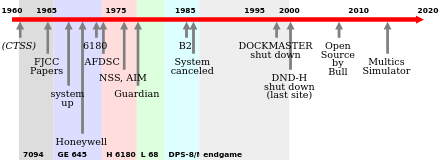
\includegraphics[scale=0.55]{images/timeline.png}
    \caption{Timeline of Multics \cite{multicians}}
    % \label{fig:my_label}
\end{figure}


\subsection{Major Goals for Multics}
\textbf{Goals for Multics are described by Corbato and Vyssotsky in \textit{Introduction and Overview of Multics System}} \cite{introductionMultics}.
\begin{itemize}
    \item Convenient remote terminal use.
    \item Continuous operation analogous to power and telephone services.
    \item A wide range of system configurations, changeable without system or user program reorganization.
    \item A high reliability internal file system.
    \item Support for selective information sharing.
    \item Hierarchical structures of information for system administration and decentralization of user activities.
    \item Support for a wide range of applications.
    \item Support for multiple programming environments and human interfaces.
    \item The ability to evolve the system with changes in technology and in user aspirations.
\end{itemize}

The team's ambition was that Multics would change the way people used and programmed computers.
\newline
\begin{displayquote}
"One of the great unanticipated discoveries of Project MAC was that 
when more than one person can use a computer at the same time, those people will
use the computer to communicate with each other." 
\textbf{Simson Garfinkel, Architects of the Information Society}
\end{displayquote}
